% =====================================================================
%  VietForces — A4 Product Brochure (1 trang)
%
%  Dịch với XeLaTeX (khuyên dùng) hoặc pdfLaTeX.
%  Đây là trang tóm tắt bắt buộc nộp kèm báo cáo.
% =====================================================================
\documentclass[11pt,a4paper]{article}

\usepackage{iftex}
\ifPDFTeX
  \usepackage[utf8]{inputenc}
  \usepackage[T5]{fontenc}
  \usepackage{lmodern}
\else
  \usepackage{fontspec}
  \setmainfont{TeX Gyre Heros}[BoldFont={TeX Gyre Heros Bold}]
  \setmonofont{DejaVu Sans Mono}[Scale=0.78]
\fi

\usepackage[a4paper, top=1.0cm, bottom=1.0cm, left=1.2cm, right=1.2cm]{geometry}
\usepackage{xcolor}
\usepackage{graphicx}
\usepackage{tikz}
\usetikzlibrary{shapes.geometric, positioning, calc, fit, backgrounds}
\usepackage{tcolorbox}
\tcbuselibrary{skins, breakable, raster}
\usepackage{enumitem}
\usepackage{multicol}
\usepackage{array}
\usepackage{booktabs}
\usepackage[hidelinks]{hyperref}

\pagestyle{empty}

% ---- colours ----
\definecolor{vfred}{HTML}{C62828}
\definecolor{vfblue}{HTML}{1565C0}
\definecolor{vfgreen}{HTML}{2E7D32}
\definecolor{vforange}{HTML}{E65100}
\definecolor{vfgold}{HTML}{F57F17}
\definecolor{vfgray}{HTML}{424242}
\definecolor{vflightgray}{HTML}{F5F5F5}
\definecolor{vflightred}{HTML}{FFEBEE}
\definecolor{vflightblue}{HTML}{E3F2FD}
\definecolor{vflightgreen}{HTML}{E8F5E9}
\definecolor{vflightorange}{HTML}{FFF3E0}

\setlist{noitemsep, topsep=2pt}

% =====================================================================
\begin{document}

% ============================================================
% HEADER — Logo + Title + Tagline
% ============================================================
\begin{tcolorbox}[
  enhanced, arc=0pt, outer arc=0pt,
  colback=vfred, colframe=vfred,
  left=6pt, right=6pt, top=6pt, bottom=6pt
]
\noindent
\begin{minipage}[c]{0.18\linewidth}
  \centering
  \begin{tikzpicture}
    \node[circle, fill=white, minimum size=1.6cm, inner sep=0pt] (logo) {
      \textcolor{vfred}{\textbf{\Large VF}}
    };
  \end{tikzpicture}
\end{minipage}%
\begin{minipage}[c]{0.58\linewidth}
  \textcolor{white}{\fontsize{22}{24}\bfseries VietForces}\\[2pt]
  \textcolor{white!85}{\large Học tiếng Việt qua trò chơi — có AI đồng hành}\\[2pt]
  \textcolor{white!70}{\small Android App $\cdot$ Web Admin $\cdot$ AI Powered $\cdot$ Real-time Leaderboard}
\end{minipage}%
\begin{minipage}[c]{0.24\linewidth}
  \centering
  \textcolor{white}{\footnotesize\textbf{Đồ án Tốt nghiệp}}\\[3pt]
  \begin{tikzpicture}
    \node[rectangle, rounded corners=3pt, fill=white, text=vfred,
          font=\footnotesize\bfseries, inner sep=4pt] {Bao $\cdot$ An $\cdot$ Hùng Cường};
  \end{tikzpicture}
\end{minipage}
\end{tcolorbox}

\vspace{4pt}

% ============================================================
% ROW 1: Goal + Stack
% ============================================================
\begin{tcbraster}[raster columns=2, raster column skip=4pt, raster row skip=4pt,
  raster equal height=rows]

% --- Mục tiêu / Goal ---
\begin{tcolorbox}[enhanced, arc=3pt, colback=vflightred, colframe=vfred,
  title={\textcolor{white}{\textbf{Mục tiêu đề tài}}}, fonttitle=\small\bfseries,
  coltitle=white, attach boxed title to top left={yshift=-2mm, xshift=4mm},
  boxed title style={colback=vfred, arc=2pt},
  left=6pt, right=6pt, top=8pt, bottom=4pt]

{\small\textbf{Vấn đề:}} {\small Thiếu ứng dụng học tiếng Việt có gamification, AI, và cộng đồng.}

\vspace{4pt}
{\small\textbf{Giải pháp:}} {\small Xây dựng hệ thống học từ vựng đa nền tảng kết hợp:}
\begin{itemize}[leftmargin=12pt]
  \item[\textcolor{vfred}{\small$\bullet$}] {\small 8 game modes tương tác để học từ vựng tiếng Việt}
  \item[\textcolor{vfred}{\small$\bullet$}] {\small AI (LLM) để luyện hội thoại và chấm bài viết}
  \item[\textcolor{vfred}{\small$\bullet$}] {\small Hệ thống streak + ELO + daily challenge duy trì thói quen học}
  \item[\textcolor{vfred}{\small$\bullet$}] {\small Cộng đồng qua leaderboard real-time và social features}
\end{itemize}
\vspace{2pt}
{\small \textbf{Đối tượng:} Người học tiếng Việt (nước ngoài, trẻ em) \& quản trị viên nội dung.}
\end{tcolorbox}

% --- Tech Stack ---
\begin{tcolorbox}[enhanced, arc=3pt, colback=vflightblue, colframe=vfblue,
  title={\textcolor{white}{\textbf{Tech Stack}}}, fonttitle=\small\bfseries,
  coltitle=white, attach boxed title to top left={yshift=-2mm, xshift=4mm},
  boxed title style={colback=vfblue, arc=2pt},
  left=6pt, right=6pt, top=8pt, bottom=4pt]

\begin{tabular}{@{}p{2.8cm}p{5cm}@{}}
\small\textbf{Android} & \small Kotlin 2.0 $\cdot$ Jetpack Compose $\cdot$ Hilt DI $\cdot$ Supabase SDK \\[2pt]
\small\textbf{Backend} & \small Supabase (PostgreSQL + Auth + Realtime + Storage) \\[2pt]
\small\textbf{Edge Fn} & \small Deno $\cdot$ 4 functions: AI proxy, streak reminder, daily challenge gen \\[2pt]
\small\textbf{Web} & \small Next.js 15 App Router $\cdot$ TypeScript $\cdot$ Tailwind CSS \\[2pt]
\small\textbf{AI} & \small OpenAI \texttt{gpt-4o-mini} qua Edge Function proxy \\[2pt]
\small\textbf{Notif} & \small Firebase Cloud Messaging (FCM) \\[2pt]
\small\textbf{Deploy} & \small Vercel (web) $\cdot$ Supabase Cloud \\
\end{tabular}
\end{tcolorbox}

\end{tcbraster}

\vspace{4pt}

% ============================================================
% ROW 2: Main Features (4 boxes)
% ============================================================
\begin{tcbraster}[raster columns=4, raster column skip=4pt, raster row skip=4pt,
  raster equal height=rows]

\begin{tcolorbox}[enhanced, arc=3pt, colback=vflightred, colframe=vfred,
  fonttitle=\footnotesize\bfseries, coltitle=white,
  title={8 Game Modes},
  attach boxed title to top left={yshift=-2mm, xshift=3mm},
  boxed title style={colback=vfred, arc=2pt},
  left=5pt, right=5pt, top=7pt, bottom=4pt]
{\scriptsize
\textbf{1.} ImageToWord\\
\textbf{2.} WordToImage\\
\textbf{3.} SyllableMatch\\
\textbf{4.} WordSearch\\
\textbf{5.} FillBlank\\
\textbf{6.} WordChain\\
\textbf{7.} SentenceOrder\\
\textbf{8.} Writing Practice\\[3pt]
100+ từ / 8 chủ đề}
\end{tcolorbox}

\begin{tcolorbox}[enhanced, arc=3pt, colback=vflightorange, colframe=vforange,
  fonttitle=\footnotesize\bfseries, coltitle=white,
  title={AI Features},
  attach boxed title to top left={yshift=-2mm, xshift=3mm},
  boxed title style={colback=vforange, arc=2pt},
  left=5pt, right=5pt, top=7pt, bottom=4pt]
{\scriptsize
\textcolor{vforange}{\textbf{5 tính năng AI:}}\\[2pt]
$\bullet$ Writing Grading\\
(chấm + gợi ý bản viết lại)\\[2pt]
$\bullet$ Open-answer Grading\\
(chấp nhận sai dấu/nghĩa đúng)\\[2pt]
$\bullet$ Mascot Reactions\\[2pt]
$\bullet$ Learning Path\\
(phân tích điểm yếu)\\[2pt]
$\bullet$ \textbf{Roleplay Tutor}\\
(hội thoại thực tế 15 tình huống)}
\end{tcolorbox}

\begin{tcolorbox}[enhanced, arc=3pt, colback=vflightgreen, colframe=vfgreen,
  fonttitle=\footnotesize\bfseries, coltitle=white,
  title={Gamification},
  attach boxed title to top left={yshift=-2mm, xshift=3mm},
  boxed title style={colback=vfgreen, arc=2pt},
  left=5pt, right=5pt, top=7pt, bottom=4pt]
{\scriptsize
\textcolor{vfgreen}{\textbf{ELO Ranking:}}\\
Bronze $\to$ Silver $\to$ Gold\\
$\to$ Platinum $\to$ Diamond\\[3pt]
\textcolor{vfgreen}{\textbf{Streak System:}}\\
+ Streak Freeze tự động\\
+ Streak Reminder (FCM)\\[3pt]
\textcolor{vfgreen}{\textbf{Daily Challenge:}}\\
Server-generated 00:00 UTC\\
+50 ELO bonus\\[3pt]
\textcolor{vfgreen}{\textbf{Leaderboard:}}\\
Real-time (Supabase Realtime)}
\end{tcolorbox}

\begin{tcolorbox}[enhanced, arc=3pt, colback=vflightblue, colframe=vfblue,
  fonttitle=\footnotesize\bfseries, coltitle=white,
  title={Security \& Quality},
  attach boxed title to top left={yshift=-2mm, xshift=3mm},
  boxed title style={colback=vfblue, arc=2pt},
  left=5pt, right=5pt, top=7pt, bottom=4pt]
{\scriptsize
\textcolor{vfblue}{\textbf{RLS on all tables:}}\\
Mỗi user chỉ đọc/ghi data của mình\\[3pt]
\textcolor{vfblue}{\textbf{SECURITY DEFINER fn:}}\\
ELO tính server-side, check \texttt{auth.uid()}\\[3pt]
\textcolor{vfblue}{\textbf{API key safe:}}\\
OpenAI key ở Supabase env vars\\
Không có trong APK\\[3pt]
\textcolor{vfblue}{\textbf{Graceful fallback:}}\\
App chạy được dù AI lỗi\\[3pt]
\textcolor{vfblue}{\textbf{Architecture:}}\\
MVVM + Repository + Hilt DI}
\end{tcolorbox}

\end{tcbraster}

\vspace{4pt}

% ============================================================
% ROW 3: Architecture mini-diagram + Social + Admin
% ============================================================
\begin{tcbraster}[raster columns=3, raster column skip=4pt, raster row skip=4pt,
  raster equal height=rows]

% --- Architecture diagram ---
\begin{tcolorbox}[enhanced, arc=3pt, colback=white, colframe=vfgray!50,
  title={\small\textbf{Kiến trúc hệ thống}}, fonttitle=\small\bfseries,
  left=4pt, right=4pt, top=6pt, bottom=4pt]
\centering
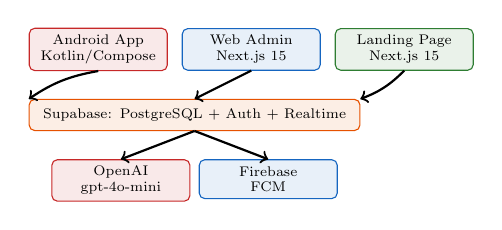
\begin{tikzpicture}[scale=0.72, transform shape, node distance=0.35cm]
  \tikzset{
    box/.style={rectangle, rounded corners=2pt, draw=#1, fill=#1!10,
      font=\scriptsize, align=center, minimum height=0.55cm, text width=2.2cm},
  }
  \node[box=vfred]  (a) {Android App\\Kotlin/Compose};
  \node[box=vfblue, right=0.25cm of a] (w) {Web Admin\\Next.js 15};
  \node[box=vfgreen, right=0.25cm of w] (l) {Landing Page\\Next.js 15};
  \node[box=vforange, below=0.5cm of w, text width=5.6cm, xshift=-1.0cm]
        (s) {Supabase: PostgreSQL + Auth + Realtime};
  \node[box=vfred, below=0.5cm of s, xshift=-1.3cm] (o) {OpenAI\\gpt-4o-mini};
  \node[box=vfblue, below=0.5cm of s, xshift=1.3cm] (f) {Firebase\\FCM};

  \draw[->, thick] (a.south) to[bend right=12] (s.north west);
  \draw[->, thick] (w.south) -- (s.north);
  \draw[->, thick] (l.south) to[bend left=12] (s.north east);
  \draw[->, thick] (s.south) -- (o.north);
  \draw[->, thick] (s.south) -- (f.north);
\end{tikzpicture}
\end{tcolorbox}

% --- Social Features ---
\begin{tcolorbox}[enhanced, arc=3pt, colback=vflightorange, colframe=vforange,
  title={\small\textbf{Social Features}}, fonttitle=\small\bfseries, coltitle=white,
  coltitle=white, attach boxed title to top left={yshift=-2mm, xshift=4mm},
  boxed title style={colback=vforange, arc=2pt},
  left=5pt, right=5pt, top=8pt, bottom=4pt]
{\small
\begin{itemize}[leftmargin=10pt]
  \item[\textcolor{vforange}{$\bullet$}] Asymmetric follow (như Twitter)
  \item[\textcolor{vforange}{$\bullet$}] Friends tab trong Leaderboard
  \item[\textcolor{vforange}{$\bullet$}] Activity feed bạn bè
  \item[\textcolor{vforange}{$\bullet$}] Xem public profile người khác
  \item[\textcolor{vforange}{$\bullet$}] Search user theo username
\end{itemize}
}
\end{tcolorbox}

% --- Admin + Deploy ---
\begin{tcolorbox}[enhanced, arc=3pt, colback=vflightblue, colframe=vfblue,
  title={\small\textbf{Web Admin Dashboard}}, fonttitle=\small\bfseries, coltitle=white,
  coltitle=white, attach boxed title to top left={yshift=-2mm, xshift=4mm},
  boxed title style={colback=vfblue, arc=2pt},
  left=5pt, right=5pt, top=8pt, bottom=4pt]
{\small
\begin{itemize}[leftmargin=10pt]
  \item[\textcolor{vfblue}{$\bullet$}] Vocabulary CRUD + image upload
  \item[\textcolor{vfblue}{$\bullet$}] User management (ban/unban)
  \item[\textcolor{vfblue}{$\bullet$}] Analytics: DAU, retention
  \item[\textcolor{vfblue}{$\bullet$}] Daily challenge scheduling
  \item[\textcolor{vfblue}{$\bullet$}] Deploy trên Vercel
\end{itemize}
}
\end{tcolorbox}

\end{tcbraster}

\vspace{4pt}

% ============================================================
% FOOTER
% ============================================================
\begin{tcolorbox}[enhanced, arc=0pt, outer arc=0pt,
  colback=vfgray, colframe=vfgray,
  left=6pt, right=6pt, top=4pt, bottom=4pt]
\noindent
\begin{minipage}[c]{0.35\linewidth}
  \textcolor{white}{\footnotesize \textbf{VietForces} — Gamified Vietnamese Learning App}\\
  \textcolor{white!75}{\scriptsize Đồ án Tốt nghiệp $\cdot$ Bao, An, Hùng Cường}
\end{minipage}%
\hfill
\begin{minipage}[c]{0.30\linewidth}
  \centering
  
\begin{tikzpicture}[node distance=0.1cm]
    \node[rectangle, rounded corners=2pt, fill=vfred!80, text=white,
          font=\scriptsize\bfseries, inner sep=3pt] (a) {Android};
    \node[rectangle, rounded corners=2pt, fill=vfblue!80, text=white,
          font=\scriptsize\bfseries, inner sep=3pt, right=0.2cm of a] (w) {Web};
    \node[rectangle, rounded corners=2pt, fill=vfgreen!80, text=white,
          font=\scriptsize\bfseries, inner sep=3pt, right=0.2cm of w] (ai) {AI};
    \node[rectangle, rounded corners=2pt, fill=vforange!80, text=white,
          font=\scriptsize\bfseries, inner sep=3pt, right=0.2cm of ai] (rt) {Realtime};
  \end{tikzpicture}
\end{minipage}%
\hfill
\begin{minipage}[c]{0.30\linewidth}
  \raggedleft
  \textcolor{white}{\scriptsize \textbf{Source:} github.com/tranthebaobnnn-ai/vietforces}\\
  \textcolor{white!75}{\scriptsize Trường ĐH KHTN — ĐHQG TP.HCM}
\end{minipage}
\end{tcolorbox}

\end{document}
